\chapter{Especificación del sistema}
	
	En los capítulos anteriores se ha proporcionado una visión general del problema a resolver. En este capítulo, dedicado a la especificación, se va a detallar el funcionamiento del algoritmo de regresión ordinal basado en redes neuronales artificiales y se realizará un análisis del coste computacional de sus fases atendiendo a posibles optimizaciones.
	
	\section{Algoritmo de Regresión Ordinal ORNNet}
	
		En esta sección se explicará el funcionamiento detallado del algoritmo a implementar.\\
		
		El modelo de la red neuronal se basa en una capa de entrada, dos capas ocultas y una capa de salida. La capa de entrada tomará los valores de entrenamiento de entrada ($x_1, x_2, ..., x_i$) que para pasar a la siguiente capa obtendrá nuevos valores ($B_1, B_2, ..., B_i$), cambiando los valores de los pesos ($w_1, w_2, ..., w_i$). Para actualizar estos valores se utilizará una función de transferencia (sigmoide), por ejemplo, una \textit{logsig} o \textit{tansig}. La primera capa oculta obtendrá los nuevos valores a partir de los datos elegidos, en cambio, la segunda capa oculta, que tendrá solo una neurona, obtendrá los valores de la capa anterior y no tendrá \textit{bias}. Esta capa tendrá como función de transferencia fija del tipo \textit{purelin}. Por último, para obtener los valores de la capa de salida, que tendrá el mismo número de neuronas que la capa de entrada, se pondrá el valor de los pesos fijo a 1 y se utilizará la función de transferencia \textit{logsig}. Una de las condiciones que hay para la capa de salida es que el valor de las \textit{bias} tiene que mantener el orden, es decir, $\beta^1_0< \beta^2_0< \cdots < \beta^{J-1}_0$. Una vez obtenida la salida se hará una transformación de los valores para poder tratarlos.\\
		
		La Figura \ref{fig:ORNNet} muestra gráficamente dicho funcionamiento.\\
		
		\begin{figure}[h]
			\centering
			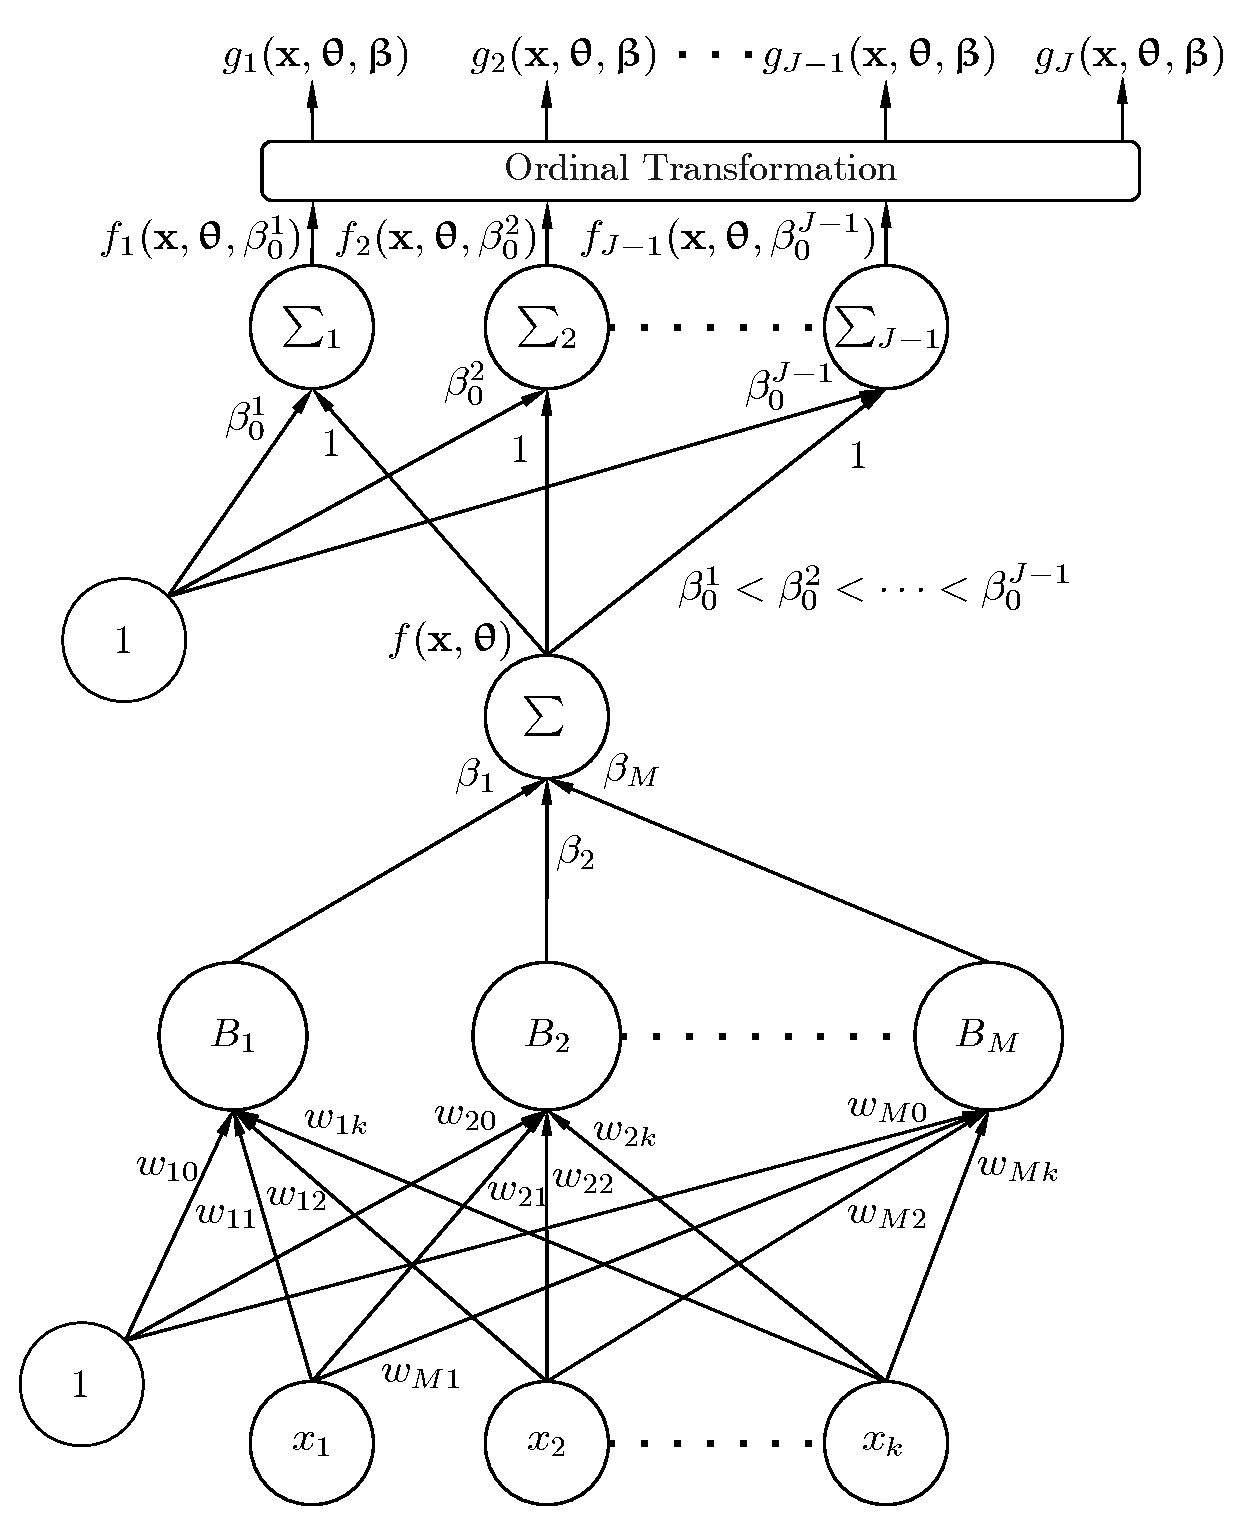
\includegraphics[scale=0.5]{img/ORNNet.pdf}
			\caption{Funcionamiento del algoritmo para redes neuronales artificiales ORNNet.}
			\label{fig:ORNNet}
		\end{figure}
		
		La mayoría de los modelos de regresión ordinal se representan como en la ecuación \ref{GeneralOR}.\\
		
		\begin{equation}
			C(\mathbf{x})=
			\begin{cases}
				c_1, & \text{si $f(\mathbf{x},{\boldsymbol \theta})\le \beta^1_0$}\\
				c_2, & \text{si $\beta^1_0<f(\mathbf{x},{\boldsymbol \theta})\le \beta^2_0$}\\
				\cdots\\
				c_J, & \text{si $f(\mathbf{x},{\boldsymbol \theta})>\beta^{J-1}_0$}
			\end{cases}
			\label{GeneralOR}
		\end{equation}\\

		siendo $c_1, c_2, ..., c_J$ las clases ordenadas, $\beta^1_0< \beta^2_0< \cdots < \beta^{J-1}_0$ los sesgos o \textit{bias} de las funciones discriminantes y $f(\mathbf{x},{\boldsymbol \theta})$ la función de ranking discriminante (en este caso, no lineal).\\
		
		Nuestro modelo, que llamaremos ORNNet, es similar al modelo POM\footnote{Proportional Odds Model, modelo explicado en el capítulo de Antecedentes.}, pero usando transformaciones básicas no lineales de las entradas en lugar de las variables de entrada. De este modo, las funciones discriminantes a utilizar son ahora:\\
		
		\begin{equation}
			f_l(\mathbf{x},{\boldsymbol \theta},\beta^l_0)=f(\mathbf{x},{\boldsymbol \theta})-\beta^l_0;\;1\le l\le J-1
			\label{funcion_modelo}
		\end{equation}\\
		
		siendo $f(\mathbf{x},{\boldsymbol \theta})$ la función de base del modelo, como por ejemplo, un sumatorio de transformaciones no lineales de las variables de entrada:\\
		
		\begin{equation}
			f(\mathbf{x},{\boldsymbol \theta})=\sum_{i=1}^M \beta_i B_i(\mathbf{x},\mathbf{w}_i)
			\label{NL}
		\end{equation}\\
		
		donde $B_i(x,w_i)$ son las funciones de base, que este proyectos se han utilizado del tipo \textit{logsig}, \textit{tansig} y \textit{purelin}.\\
		
		Haciendo uso del modelo POM, las probabilidades acumuladas, las posibilidades acumuladas\footnote{Cumulative odds.} y los logits acumulados serían:\\
		
		\begin{eqnarray}
			P(Y\le l) = p_1+\cdots+p_l \\
			odds(Y\le l) =\frac{P(Y\le l)}{1-P(Y\le l)}\\
			logit(Y\le l)=\ln \left(\frac{P(Y\le l)}{1-P(Y\le l)}\right)
			\label{POM_odds}
		\end{eqnarray}\\
		
		para $1\le l\le J-1$.\\

		Y en el modelo de ORNNet:\\
		
		\begin{eqnarray}
			& logit(Y\le l)=f_l(\mathbf{x},{\boldsymbol \theta},\beta^l_0)=f(\mathbf{x},{\boldsymbol \theta})-\beta^l_0;\; & 1\le l\le J-1\\
			& P(Y\le l)=\frac{1}{1+\exp(f(\mathbf{x},{\boldsymbol \theta)}-\beta^l_0)};\; & 1\le l\le J-1\\
			& P(Y\le J)=1 & 
			\label{ORNNet_odds}
		\end{eqnarray}\\

		Esto permite expresar las probabilidades como:\\
		
		\begin{eqnarray}
			& P(Y=1)=g_{1}(\mathbf{x},\boldsymbol{\theta},{\boldsymbol \beta})=P(Y\le 1) \\
			& P(Y=l)=g_{l}(\mathbf{x},\boldsymbol{\theta},{\boldsymbol \beta})=P(Y\le l)-P(Y\le l-1)
			\label{probability}
		\end{eqnarray}\\
		
		donde $2 \leq l \leq J$.\\
		
		En el problema de clasificación ordinal, la medidas $x_{i}$, $i=1,2,...,k$, se toman de manera individual (o como un objeto) y éstos se clasifican en una de las $J$ clases en base a dichas mediciones. Se asume que $J$ es finito y que las medidas de $x_{i}$ son observaciones aleatorias de esas clases.\\
		
		Sea $D = \left\{(\mathbf{x}_{n}, \mathbf{y}_{n}); n=1,2,...,N\right\}$ un conjunto de datos de entrenamiento, donde $\mathbf{x}_{n} =(x_{1n},...,x_{kn})$ es el vector de mediciones tomando valores en $\mathbf{\Omega} \subset {\mathbb R}^{k}$, e $\mathbf{y}_{n}$ el nivel de clase o etiqueta del $n$-ésimo individuo. Se adoptará la técnica más común para representar niveles de clases usando un vector de codificación ``$1$-de-$J$'', $\mathbf{y}=\left(y^{(1)} ,y^{(2)} ,...,y^{(J)} \right)$, tal que $y^{(l)} =1$ si $\mathbf{x}$ corresponde a un elemento perteneciente a la clase $l$ y, en otro caso, a $y^{(l)} =0$.\\
		
		La función que se usará para evaluar una red ORNNet es la del error cuadrático medio (MSE) que viene expresada a continuación:\\
		
		\begin{eqnarray}
			l(\boldsymbol{\beta},\boldsymbol{\theta})=-\frac{1}{N}\sum_{n=1}^N \sum_{l=1}^J \left( g_{l}(\mathbf{x},\boldsymbol{\theta},{\boldsymbol \beta})-y_n^{(l)}\right)^2
			\label{eq:mse}
		\end{eqnarray}\\
		
		donde $\boldsymbol{\beta}=(\beta_0^1,...,\beta_0^{J-1})$ es el vector de sesgos o \textit{bias} y el modelo es:\\
		
		\begin{eqnarray}
			g_{1}(\mathbf{x},\boldsymbol{\theta},{\boldsymbol \beta})= \displaystyle \frac{1}{1+\exp(f_1(\mathbf{x},{\boldsymbol \theta},\beta^1_0))} \\
			g_{l}(\mathbf{x},\boldsymbol{\theta},{\boldsymbol \beta})= \displaystyle \frac{1}{1+\exp(f_l(\mathbf{x},{\boldsymbol \theta},\beta^l_0))}-\frac{1}{1+\exp(f_{l-1}(\mathbf{x},{\boldsymbol \theta},\beta^{l-1}_0))}  \\
			g_{J}(\mathbf{x},\boldsymbol{\theta},{\boldsymbol \beta})= \displaystyle 1-\frac{1}{1+\exp(f_{J-1}(\mathbf{x},{\boldsymbol \theta},\beta^{J-1}_0))}
			\label{modelo}
		\end{eqnarray}\\
		
		donde $l = 2,\dots,J-1$.\\
		
		Para el propósito que de este algoritmo, se ha realizado una adaptación del procedimiento para óptimos locales en regresión ordinal, $iRprop^{+}$, y la función del MSE (Ecuación \ref{eq:mse}). En este caso, el vector gradiente sigue la siguiente formulación.\\
		
		\begin{equation}
			\nabla l(\boldsymbol{\beta},\beta_1,\cdots,\beta_M, \mathbf{w}_1,\cdots,\mathbf{w}_M) = \left(\frac{\partial l}{\partial \boldsymbol{\beta}},\frac{\partial l}{\partial \beta_1},\cdots,\frac{\partial l}{\partial \beta_M},\frac{\partial l}{\partial \mathbf{w}_1},\cdots, \frac{\partial l}{\partial \mathbf{w}_M} \right) \nonumber
			\label{gradient_vector}
		\end{equation}\\
		
		donde $\beta_1,...,\beta_M$ y $w_1,...,w_M$ son los coeficientes de la función de base mostrada en la Figura \ref{fig:ORNNet}.\\

		Siendo $\eta$ alguno de los parámetros $\boldsymbol{\beta}$ o $\boldsymbol{\theta}$. Con lo que:\\
		
		\begin{eqnarray*}
			\frac{\partial l}{\partial \eta} & = &  \frac{1}{N} \sum_{n=1}^{N} \sum_{l=1}^{J} 2\cdot\left( g_{l}(\mathbf{x},\boldsymbol{\theta},{\boldsymbol \beta})-y_n^{(l)}\right)\cdot\frac{\partial g_l(\mathbf{x},{\boldsymbol \theta},{\boldsymbol \beta})}{\partial \eta}. \nonumber
			\label{derivada}
		\end{eqnarray*}\\
		
		Derivando ahora la función $g$:\\
		
		\begin{eqnarray*}
			\frac{\partial g_l(\mathbf{x},{\boldsymbol \theta},{\boldsymbol \beta})}{\partial \eta} & = &
			\begin{cases}
				\displaystyle \left( \frac{-e^{f_{1}}}{\left( 1+ e^{f_{1}} \right)^2}\right) \frac{\partial f_{1}}{\partial \eta},& l=1 \\
				\displaystyle \left( \frac{-e^{f_{l}}}{\left( 1+ e^{f_{l}} \right)^2}\right) \frac{\partial f_{l}}{\partial \eta} -\left( \frac{-e^{f_{l-1}}}{\left( 1+ e^{f_{l-1}} \right)^2}\right) \frac{\partial f_{l-1}}{\partial \eta}, & l=2,\cdots,J-1\\
				\displaystyle -\left( \frac{-e^{f_{J-1}}}{\left( 1+ e^{f_{J-1}} \right)^2}\right) \frac{\partial f_{J-1}}{\partial \eta}, & l=J
			\end{cases}
			\nonumber \\
			\label{derivada_g}
		\end{eqnarray*}\\
		
		donde $g_l(\mathbf{x},{\boldsymbol \theta},{\boldsymbol \beta})=g_l$ y $f_l(\mathbf{x},{\boldsymbol \theta},\beta^l_0)=f_l$.\\

		La siguiente expresión incluye las derivadas de los coeficientes para la capa de salida:\\
		
		\begin{eqnarray}
			& \displaystyle \frac{\partial f_{l}}{\partial \beta_{0}^{k}} = \left\{ \begin{array}{ll}
         0 & \mbox{$k \neq l$}\\
        -1 & \mbox{$k = l$} \end{array} \right. , \nonumber \\
& \displaystyle \frac{\partial f_{l}}{\partial \beta_{s}} = B_{s}(\mathbf{x},\mathbf{w}_s);\;1\le s\le M \nonumber
		\end{eqnarray}\\

		El gradiente para las capas ocultas dependerá del tipo de función base. Si $B_{s}(\mathbf{x},\mathbf{w}_s)$ son nodos sigmoidales; cuya ecuación es:\\
		
		\begin{eqnarray}
			B_{s}(\mathbf{x},\mathbf{w}_s) & = & \sigma\left(\sum_{i=1}^k w_{is} x_i\right), \sigma(x)=\frac{1}{1+e^{-x}}
		\end{eqnarray}\\

		Entonces,\\

		\begin{eqnarray}
			\frac{\partial l}{\partial \mathbf{w}_s} & = & \left(\frac{\partial f_{l}}{\partial w_{s1}}, \cdots, \frac{\partial f_{l}}{\partial w_{sk}}\right) \nonumber \\
			\frac{\partial f_{l}}{\partial w_{st}} & = & \beta_s^l\sigma'\left( \sum_{i=1}^k w_{is} x_i \right) x_t \nonumber
		\end{eqnarray}\\
		
		donde $l = 1, 2, \dots, J-1$, $t = 1, 2, \dots, k$ y $s = 1, 2, \dots, M$.
		
	\section{Descripción funcional del sistema}
	
		En esta sección, se describirá el sistema con detalle, haciendo uso de técnicas de modelado que mostrarán de un modo inequívoco cómo interviene el usuario en el sistema, cuáles son los ítems que componen el sistema y qué operaciones soportan estos ítems. Para ello, se empleará la metodología UML (Lenguaje Unificado de Modelado) \cite{UML}.\\
		
		UML es un lenguaje de modelado que mediante un determinado vocabulario y un conjunto de reglas es capaz de representar conceptual y físicamente un sistema. El motivo de escoger esta metodología es que incorpora técnicas sencillas que dan una visión más cercana de lo que el usuario espera obtener.
		
		\subsection{Valores de los diferentes parámetros que utiliza el sistema}

		Con respecto a los principales valores del conjunto de datos que se vaya a usar, el número de capas ocultas, las funciones de las capas ocultas, etc. serán valores que se decidirán en secciones posteriores, durante la experimentación o en cuanto se pueda evaluar el funcionamiento del módulo, de manera que se consiga una mejor solución.\\
		
		A continuación se describen los parámetros más comunes a definir por el usuario para el algoritmo o la creación de la red neuronal artificial:
		
		\begin{itemize}
			\item \textit{Conjunto de datos}: son los datos que se especificarán para que el sistema pueda funcionar y para que la red neuronal pueda entrenar y simular los resultados de salida.
			\begin{itemize}
				\item \textbf{Datos de entrada}: son los datos de entrada del sistema, éstos vendrán definidos para cada conjunto de datos con los que se pruebe el sistema y tendrán un formato ordinal.
				\item \textbf{Datos objetivos}: son los datos objetivo del sistema, éstos se utilizarán para comprobar cuanto de buena es la red neuronal y el algoritmo implementado conteniendo los resultados reales de la clasificación.
			\end{itemize}
			\item \textit{Número de neuronas en las capas ocultas}: este parámetro podrá ser variable en función de cuantas capas ocultas y cuantas neuronas se desee poner en la red neuronal, por defecto se establecerán dos capas en la que la primera capa oculta contendrá 20 neuronas por defecto y la segunda capa oculta, que será fija para el sistema, contendrá 1 neurona. Adicionalmente, se proporcionará la opción de calcular el número óptimo de neuronas que debería haber en las capas ocultas.
			\item \textit{Número de neuronas en la capa de salida}: este parámetro es fijo, ya que será el mismo número que haya en la entrada del sistema.
			\item \textit{Funciones de transferencia de las capas}: este parámetro podrá contener alguno de los siguientes valores: \textit{logsig}, \textit{tansig}, \textit{purelin}, \textit{softmax}; para las capas ocultas que se definan. Adicionalmente, para las capas fijas, la última capa de la capa oculta y la capa de salida, tendrán el valor de \textit{purelin} y \textit{logsig} respectivamente.
			\item \textit{Función de entrenamiento}: la función de entrenamiento que se usará en el sistema será la implementada para el algoritmo ORNNet que será una modificación del algoritmo visto con anterioridad iRProp+.
			\item \textit{Función de aprendizaje}: este parámetro vendrá por defecto en el sistema al crear la red neuronal y se utilizará el valor: \textit{learngdm}, la cual se basa en descenso de gradiente.
			\item \textit{Función de precisión}: para este parámetro también se usará el valor por defecto: \textit{mse}, aunque se podrá modificar en cuanto convenga. Los distintos valores que podrá tomar son: \textit{mse} y \textit{mae}.
		\end{itemize}

		\subsection{Diagramas de Casos de Uso}

		Para obtener el modelo de objetos del software a desarrollar, se partirá de un conjunto de casos de uso desde un alto nivel de abstracción hasta un nivel de detalle más elevado, pudiendo obtener de esta forma todos los requisitos necesarios y los objetos que conformarán el sistema. Un caso de uso especifica el comportamiento de un sistema o de una parte del mismo y es una descripción de un conjunto de secuencias de acciones, incluyendo variantes, que ejecuta un sistema para producir un resultado observable de valor para un actor.\\
		
		Los casos de uso se emplean para capturar el comportamiento deseado del sistema en desarrollo sin tener que especificar cómo se implementa ese comportamiento, además de proporcionar un medio para que los desarrolladores, los usuarios finales del sistema y los expertos del dominio lleguen a una comprensión común del sistema.

			\subsubsection{Perfiles de usuario}

			En el sistema de resolución de problemas de modelado se pueden distinguir distintos tipos de actores, un actor representa un conjunto coherente de roles que juegan los usuarios de los casos de uso al interactuar con él. Los actores pueden ser personas o sistemas externos, establecidos por la siguiente clasificación:
			
			\begin{itemize}
				\item \textit{Principales:} personas que usan el sistema, serán los usuarios del sistema. Este proyecto no se basa en la interacción con el usuario del sistema ya que retoma más importancia la implementación y la obtención de resultados del algoritmo propuesto, no obstante, existirá una interfaz gráfica con la que el usuario podrá interactuar. El usuario podrá ejecutar el algoritmo y obtener los resultados. Para alcanzar dicho fin, el usuario tendrá que introducir unos parámetros de entrada, es decir, un conjunto de datos de entrada y de objetivos para el entrenamiento y el testeo de la red neuronal. Una vez especificados, habrá que crear la red neuronal y seguidamente realizar el entrenamiento y la simulación de la misma. Por último, tendrá que recoger las salidas. Las personas que usarán el sistema serán aquellas que tengan conocimientos acerca del uso y funcionamiento de redes neuronales artificiales.
				\item \textit{Secundarios:} personas que mantienen o administran el sistema. El mantenimiento de esta aplicación va a ser llevada por otras personas que realicen mejoras o actualizaciones debido a evoluciones que sufra el toolbox nnet de Matlab.
				\item \textit{Material externo:} dispositivos materiales imprescindibles que forman parte del ámbito de la aplicación y deben ser utilizados.
				\item \textit{Otros sistemas:} sistemas con los que la aplicación interactúa. Sistema Operativo: indica el sistema sobre el cual trabajará la aplicación, que dado a que el lenguaje es proporcionado por Matlab y éste es multiplataforma, podrá ser cualquiera de las arquitecturas soportadas.
			\end{itemize}

			\subsubsection{Casos de Uso}
	
			El modelado de Casos de Uso es la técnica más efectiva y a la vez la más simple para modelar los requisitos del sistema desde la perspectiva del usuario. Los Casos de Uso se utilizan para modelar cómo un sistema funciona actualmente o cómo los usuarios desean que funcione. No es realmente una aproximación a la orientación a objetos, realmente es una forma de modelar procesos. Además es, sin embargo, una manera muy eficaz de dirigirse hacia el análisis de sistemas orientados a objetos, aunque en este caso no será ese su fin. Los casos de uso son, generalmente, el punto de partida del análisis con UML.\\
			
			La Figura \ref{fig:DiagramaContexto} y la Tabla \ref{tab:CU0} representan el caso de uso correspondiente al contexto del sistema.\\
			
			\begin{figure}[!h]
				\centering
				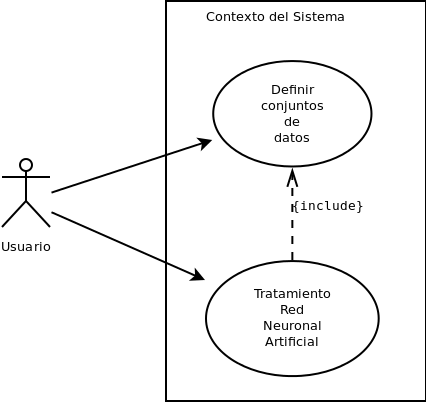
\includegraphics[scale=0.6]{uml/DiagramaContexto.png}
				\caption{Diagrama de Contexto del Sistema.}
				\label{fig:DiagramaContexto}
			\end{figure}
			
			\begin{table}[!h]
				\centering
				\begin{tabular}{l|p{.5\linewidth}}
					\hline Nombre & Contexto del Sistema. \\ 
					\hline Actores & Usuario. \\ 
					\hline Descripción & El sistema proporciona al usuario la opción de definir el conjunto de datos o de tratar la red neuronal artificial, ya sea creándola, entrenándola u obteniendo los resultados. \\ 
					\hline Casos de Uso & \textit{CU1}. \textbf{Definir el conjunto de datos}. Si el usuario quiere definir el conjunto de datos tendrá que elegir esta opción.
					
					\textit{CU2}. \textbf{Tratamiento Red Neuronal Artificial}. Si el usuario desea realizar el tratamiento de la red neuronal, ya sea crearla, entrenarla u obtener los resultados. \\ 
					\hline Flujo Principal de Eventos & El usuario comenzará eligiendo la opción que desea ejecutar, que podrá ser o definir el conjunto de datos a usar o tratar la red neuronal artificial. \\ 
					\hline 
				\end{tabular}
				\caption{Diagrama de caso de uso CU0: Contexto del Sistema.}
				\label{tab:CU0}
			\end{table}
			
			La Figura \ref{fig:CU1} y la Tabla \ref{tab:CU1} representan el caso de uso correspondiente al tratamiento de la RNA.\\
			
			\begin{figure}[!h]
				\centering
				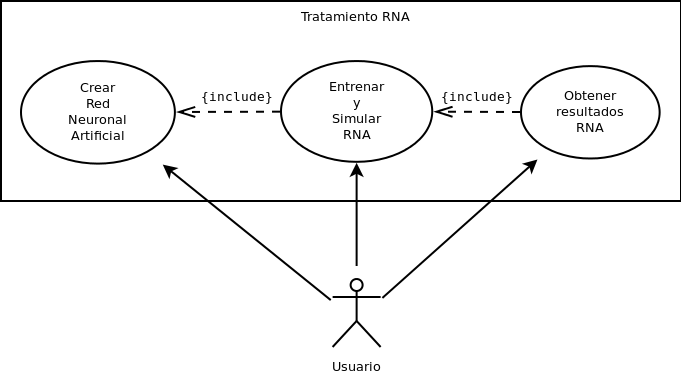
\includegraphics[scale=0.5]{uml/DiagramaNivel1.png}
				\caption{Diagrama de caso de uso CU1: Tratamiento RNA.}
				\label{fig:CU1}
			\end{figure}
			
			\begin{table}[!h]
				\centering
				\begin{tabular}{l|p{.5\linewidth}}
					\hline Nombre & Tratamiento RNA. \\ 
					\hline Actores & Usuario. \\ 
					\hline Descripción & El sistema proporciona las opciones para el tratamiento de una red neuronal artificial para regresión ordinal. \\ 
					\hline Casos de Uso & \textbf{Crear RNA}: consiste en la creación de una red neuronal artificial para regresión ordinal.
					
					\textbf{Entrenar y simular RNA}: consiste en realizar el entrenamiento de la red neuronal aplicando el algoritmo ORNNet explicado en la sección 7.1.
					
					\textbf{Obtener resultados RNA}: consiste en obtener los resultados generados por el entrenamiento y simulación del conjunto de datos en la red neuronal aplicando el algoritmo desarrollado de regresión ordinal. \\ 
					\hline Flujo Principal de Eventos & El usuario crea la red neuronal de la que, a partir de ella y del conjunto de datos cargado previamente, se realiza el entrenamiento y la simulación de la red haciendo uso del algoritmo implementado, ORNNet, del cual se obtienen los resultados para el posterior análisis de los mismos. \\ 
					\hline 
				\end{tabular}
				\caption{Diagrama de caso de uso CU1.}
				\label{tab:CU1}
			\end{table}

		\subsection{Diagrama de Secuencia}
			
			Los diagramas de Secuencia son un tipo de diagrama usados para modelar interacciones entre objetos en un sistema según UML. Un diagrama de secuencia muestra la interacción de un conjunto de objetos en una aplicación a través del tiempo y se modela para cada caso de uso. Mientras que el diagrama de casos de uso permite el modelado de una vista \textit{business} del escenario, el diagrama de secuencia contiene detalles de implementación del escenario, incluyendo los objetos y clases que se usan para implementar el escenario, y mensajes intercambiados entre los objetos.\\

			La Figura \ref{fig:secuencia} representa el diagrama de secuencia correspondiente al funcionamiento del sistema.
			
			\begin{figure}[h]
				\centering
				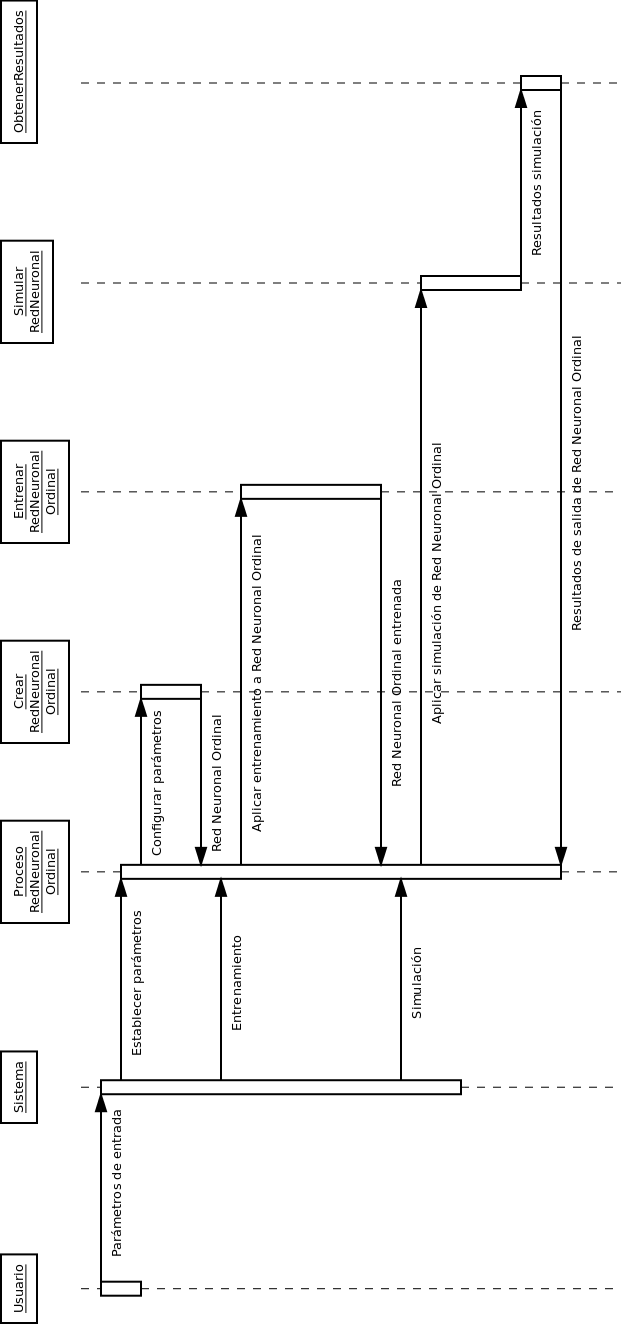
\includegraphics[scale=0.5]{uml/DiagramaSecuencia.png}
				\caption{Diagrama de Secuencia.}
				\label{fig:secuencia}
			\end{figure}
